\documentclass[a4paper,12pt]{article}

% Paquetes
\usepackage[utf8]{inputenc} % Codificación de caracteres
\usepackage[T1]{fontenc} % Salida de caracteres
\usepackage[spanish]{babel} % Idioma
\usepackage{amsmath, amssymb} % Simbolos matemáticos
\usepackage{geometry} % Ajuste de márgenes
\geometry{top=3cm, bottom=3cm, left=3cm, right=3cm}
\usepackage{graphicx} % Inclusión de gráficos
\usepackage{hyperref} % Hipervínculos
\usepackage{xcolor} % Colores

\addto\captionsspanish{\renewcommand{\tablename}{\textbf{Tabla}}}

% Título y autor
\title{Método Adam vs. SGD}
\author{}
\date{}

\begin{document}

\maketitle % Genera el título

% \tableofcontents % Tabla de contenido (opcional)
\vspace{-2cm}
\begin{table}[!ht]
    \centering
    \caption{Comparação de métodos de optimización (Head and Neck 01).}
    \vspace{0.5cm}
    \label{tab:exemplo}
    \begin{tabular}{ccc}
        \hline
        Método & Iterações & Tempo (s) \\
        \hline
        Adam & $8900$ &  $1070.26$ \\
        SGD & $28000$ & $3325.69$ \\
        \hline
    \end{tabular}
\end{table}
\vspace{-1cm}
\begin{table}[!ht]
    \centering
    \caption{Comparação de métodos de optimización (Head and Neck 02).}
    \vspace{0.5cm}
    \label{tab:exemplo}
    \begin{tabular}{ccc}
        \hline
        Método & Iterações & Tempo (s) \\
        \hline
        Adam & $12500$ &  $1171.9$ \\
        SGD & $43100$ & $4115.06$ \\
        \hline
    \end{tabular}
\end{table}
\vspace{-1cm}
\begin{table}[!ht]
    \centering
    \caption{Comparação de métodos de optimización (Head and Neck 03).}
    \vspace{0.5cm}
    \label{tab:exemplo}
    \begin{tabular}{ccc}
        \hline
        Método & Iterações & Tempo (s) \\
        \hline
        Adam & $13500$ &  $1319.48$ \\
        SGD & $44900$ & $4719,93$ \\
        \hline
    \end{tabular}
\end{table}

\vspace{-1cm}
\begin{table}[!ht]
    \centering
    \caption{Comparação de métodos de optimización (Head and Neck 04).}
    \vspace{0.5cm}
    \label{tab:exemplo}
    \begin{tabular}{ccc}
        \hline
        Método & Iterações & Tempo (s) \\
        \hline
        Adam & $14100$ &  $1586.56$ \\
        SGD & $44900$ & $4719,93$ \\
        \hline
    \end{tabular}
\end{table}

\vspace{-1cm}
\begin{table}[!ht]
    \centering
    \caption{Comparação de métodos de optimización (Head and Neck 15).}
    \vspace{0.5cm}
    \label{tab:exemplo}
    \begin{tabular}{ccc}
        \hline
        Método & Iterações & Tempo (s) \\
        \hline
        Adam & $14100$ &  $1586.56$ \\
        SGD & $44900$ & $4719,93$ \\
        \hline
    \end{tabular}
\end{table}

\begin{figure}[!ht]
    \centering
    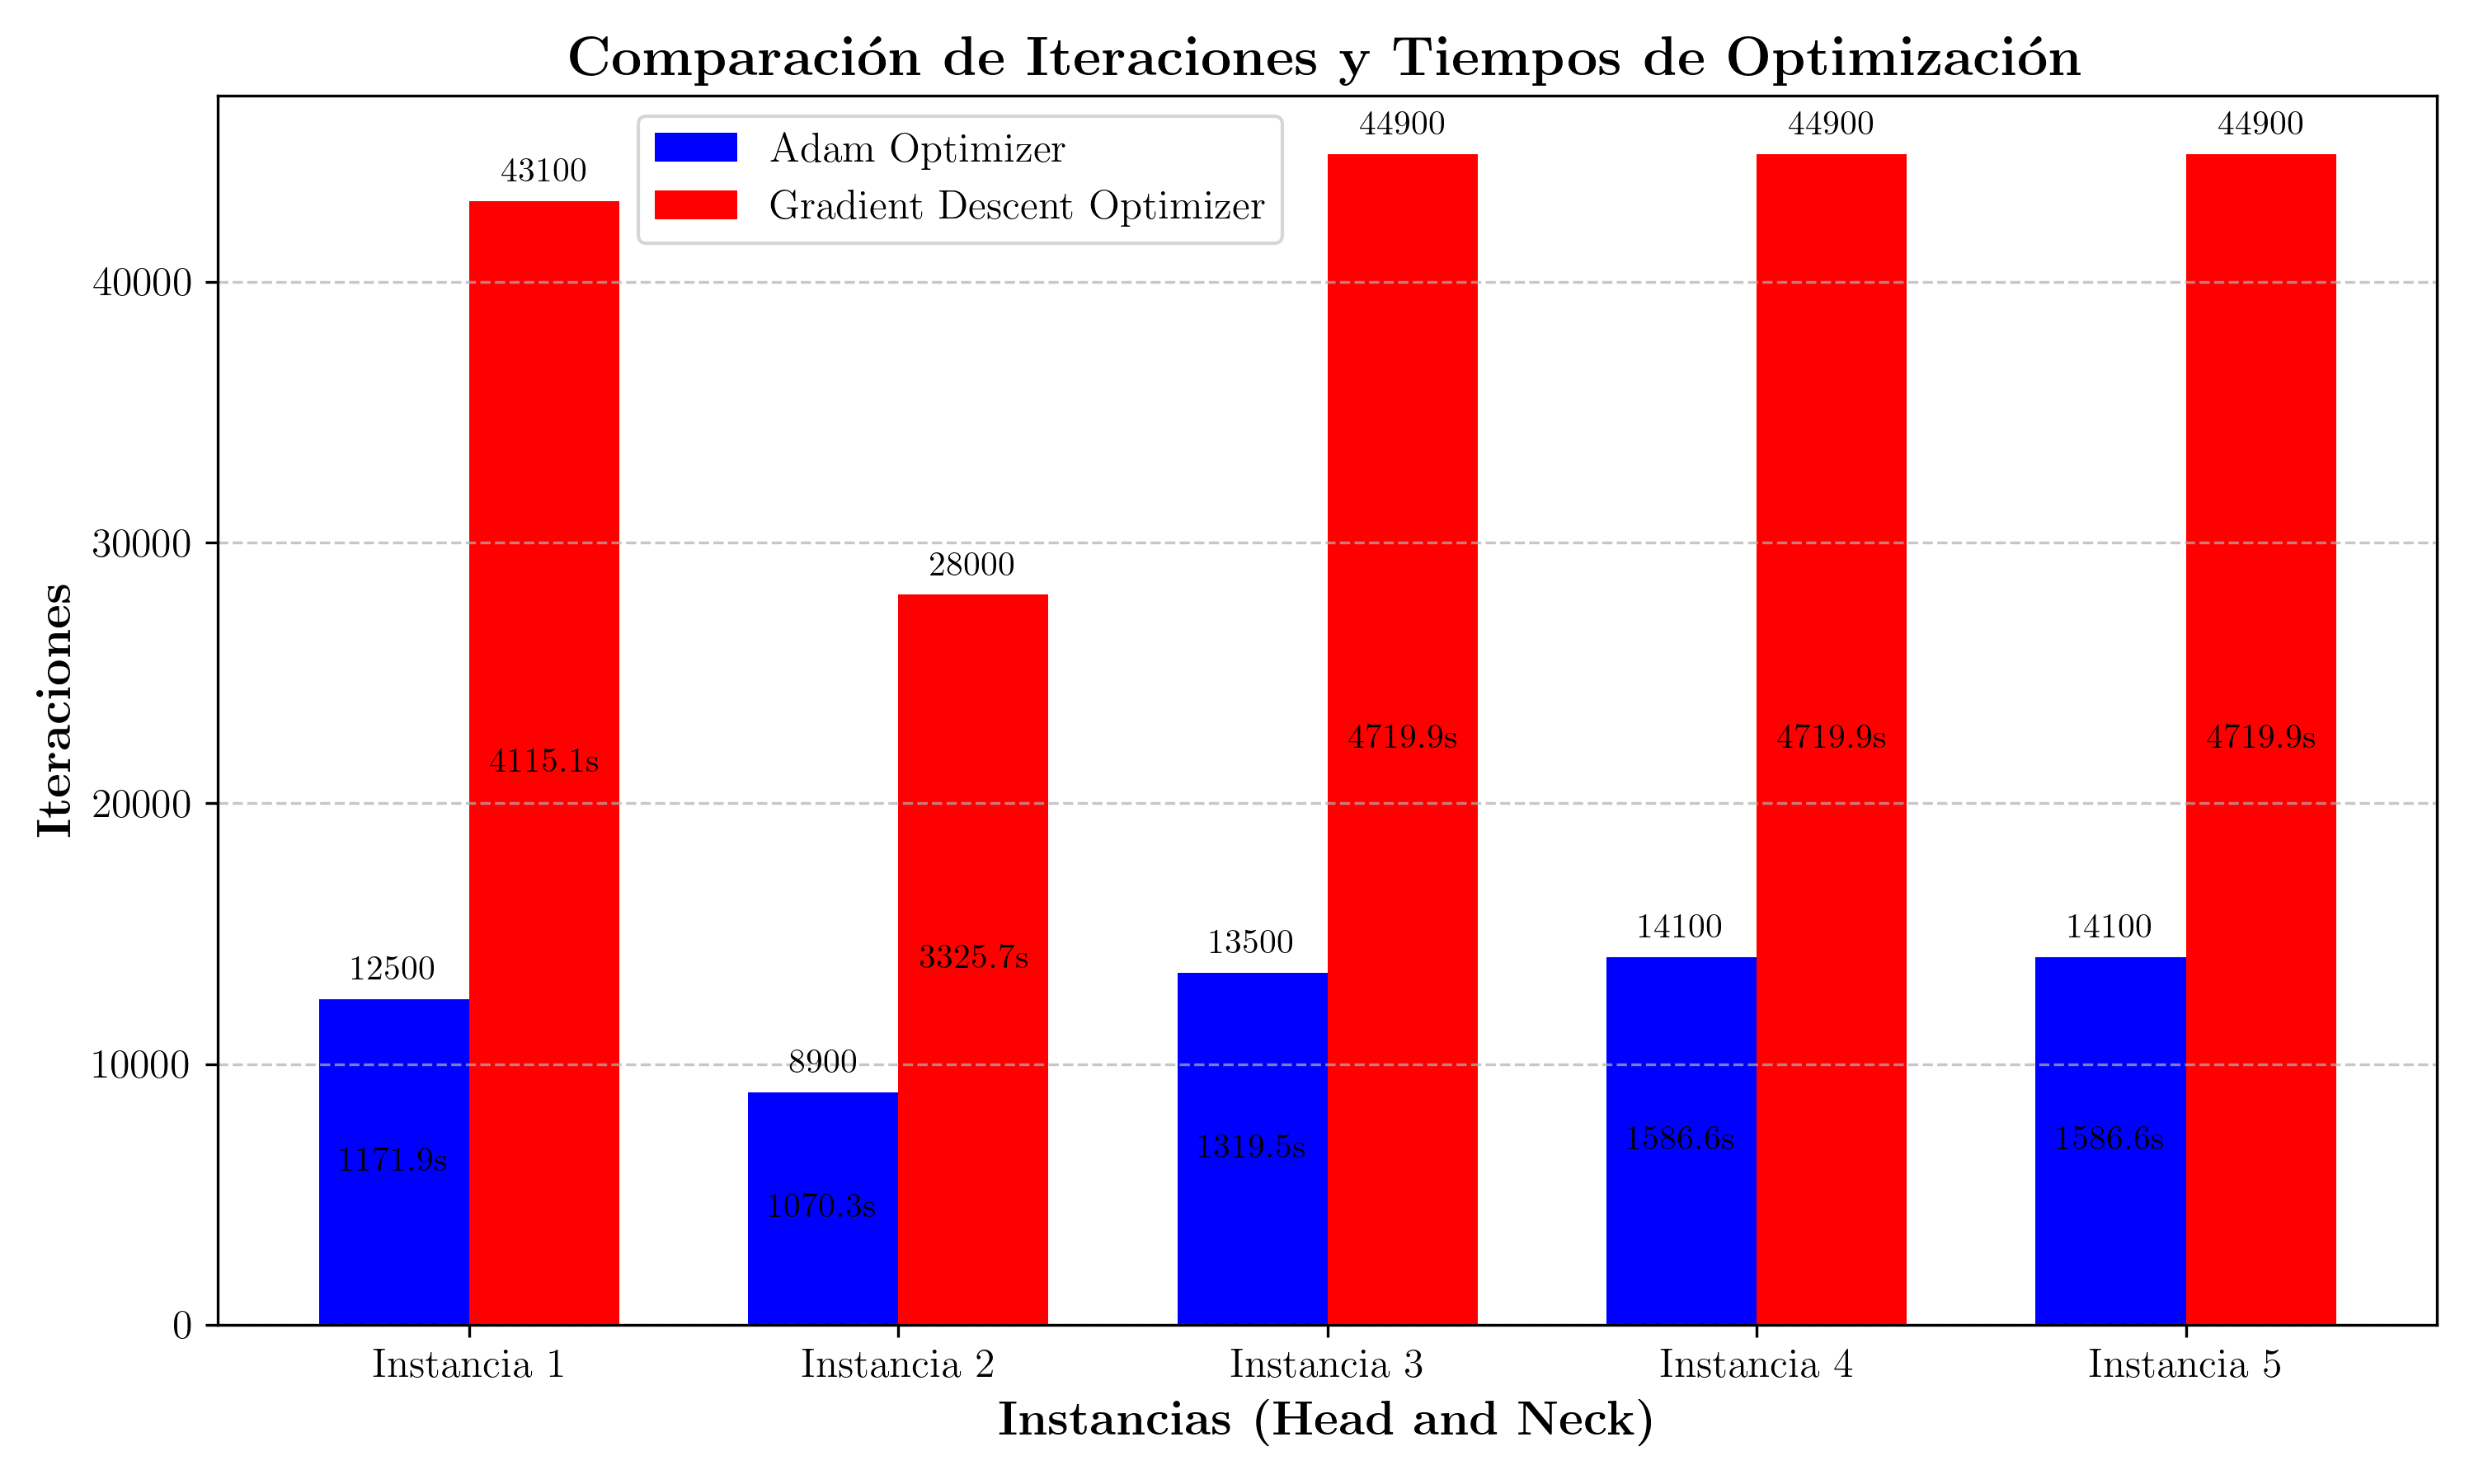
\includegraphics[width=0.9\textwidth]{../Graficos/comparacion_metodos.png}
    \caption{Método Adam vs SGD: Comparación de Iteraciones y Tiempos}
    \label{fig:exemplo}
  \end{figure}

  \begin{figure}[!ht]
    \centering
    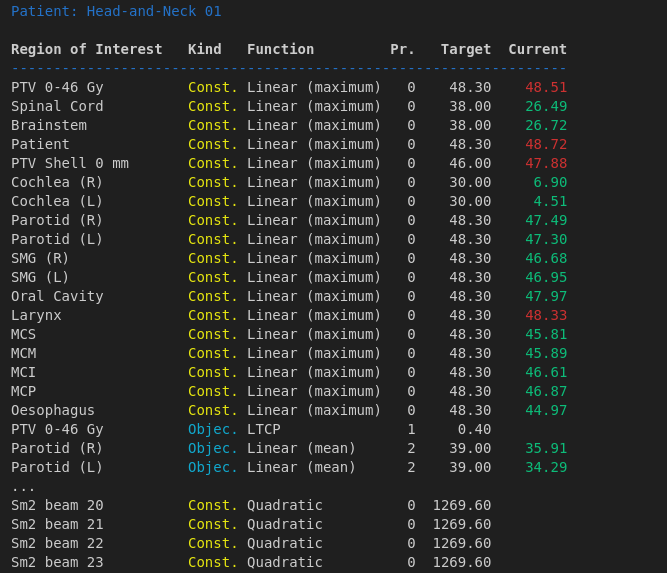
\includegraphics[width=0.9\textwidth]{result_adam01.png}
    \caption{Resultado Head and Neck 01 (Adam)}
    \label{fig:result_adam}
  \end{figure}
Los resultados presentados en la Fig.~\ref{fig:result_adam} usando el método Adam, se obtuvieron con $1800$ iteraciones y un tiempo de $221.29 $ segundos, se observa que el resultado obtenido con el método Adam es satisfactorio, ya que se logra una buena segmentación de la región de interés.

\begin{figure}[!ht]
    \centering
    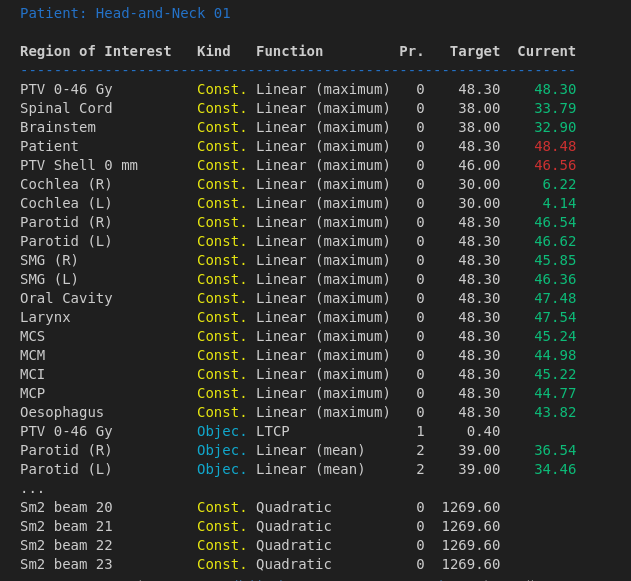
\includegraphics[width=0.9\textwidth]{result_sgd01.png}
    \caption{Resultado Head and Neck 01 (SGD)}
    \label{fig:result_sgd}
  \end{figure}
\newpage
Los resultados presentados en la Fig.~\ref{fig:result_sgd} usando el método SGD, se obtuvieron con $6200$ iteraciones y un tiempo de $729.83$ segundos, se observa que el resultado obtenido con el método Adam es satisfactorio, ya que se logra una buena segmentación de la región de interés.


\end{document}
